\documentclass[11pt]{article}
\usepackage{icmlko}
\begin{document}

\title{죽은 손잡이가 되살아났다 --- 봉우리의 자리는 자료 크기의 함수다}
\author{월드모델 실험실}
\date{노트 406 · 2026년 8월 1일}
\maketitle

\begin{abstract}
노트 216이 알파를, 216·243이 $\tau$ 를, \textbf{272가 깊이를} 죽였다.
노트 396이 $K$ 를 살릴 때 적은 이유는 ``$K$ 는 봉우리가 없는 순수 비용
손잡이''라서, 봉우리가 있는 손잡이는 안쪽에서 고르면 빗나간다는 것이었다.

노트 405가 다른 실험(원핫 대신 깊이를 주면 구멍이 메워지는가) 도중에
\textbf{깊이 $4 \to 6$ 이 판을 올리는 것}을 봤다. 미리 실패 조건을 적고
$K{=}32$ 로 관문을 돌렸다 --- \emph{$K{=}8$ 에서만 나는 이득이면 깊이의
부활이 아니라 자루의 대체물이다.}

\begin{center}
\begin{tabular}{lrr}
\hline
짝 12뽑기 $K{=}32$, 깊이6 $-$ 깊이4 & 차 & 부호 \\
\hline
\textbf{판} & $\mathbf{+0.0093 \pm 0.0039}$ & $\mathbf{12/12}$ \\
아이돌 & $+0.1179$ & $12/12$ \\
펀딩 & $+0.0409$ & $12/12$ \\
모바일 & $+0.0201$ & $12/12$ \\
게임 & $+0.0193$ & $12/12$ \\
애니 & $+0.0135$ & $12/12$ \\
\hline
\textbf{웹툰} & $\mathbf{-0.0241}$ & $0/12$ \\
\hline
\end{tabular}
\end{center}

실패 조건은 안 걸렸다. \textbf{채택했다} --- 씨앗 12평균 판이
$0.4477 \pm 0.0004 \to \mathbf{0.4659 \pm 0.0005}$ 다. 아이돌 하나가
$+0.125$ 를 낸다($0.1909 \to 0.3163$).
\end{abstract}

\section{첫 음수를 갈랐다}

웹툰은 판에서 제일 큰 도메인(유보 711)인데 관문에서 혼자 $-0.0241 \cdot 0/12$
로 거꾸로 갔다. 채택 전에 갈랐다.

\textbf{실제 자료에서는 웹툰이 $+0.0020$ 으로 오른다}($0.4900 \to 0.4920$).
관문은 학습 행을 되뽑기해서 두 팔을 짝지운다 --- 그 되뽑기에 웹툰이 유독
민감하다는 뜻이지 깊이가 웹툰을 해친다는 뜻이 아니다. \textbf{깊은 나무는
학습 표본에 대한 분산이 크고, 웹툰이 그것을 제일 크게 보인다.} 관문 수치는
그래서 \textbf{보수적인 추정}이다 --- 판도 관문에선 $+0.0093$ 인데 실제
자료에선 $+0.0182$ 다.

\section{왜 죽었던 것이 살아나나}

노트 272 이후 자료가 자랐다. 이번 사이클에만 만화 $+4{,}999$ · 웹툰 $+835$ ·
애니 $+1{,}382$ 행이 들어왔고 펀딩 표본이 위쪽 19\%만 담던 것에서 균일
표본으로 교정됐다. 학습 행은 지금 18{,}540 이다.

\textbf{봉우리의 자리는 자료 크기의 함수다.} 행이 적을 때 깊이 6 이
과적합이던 것이, 행이 늘면 과적합이 아니게 된다. 손잡이를 죽인 판정은
\textbf{그때의 자료에 대한 판정}이었지 손잡이에 대한 판정이 아니었다.

\textbf{새 규약: 죽은 손잡이는 자료가 크게 자라면 다시 잰다.} 노트 216의
알파와 216·243의 $\tau$ 는 그 뒤로 아무도 안 재 봤다.

\section{남은 것}

\begin{tabular}{lp{7.2cm}}
\hline
알파와 $\tau$ & 같은 이유로 다시 쓸어야 한다 \\
무릎이 정말 6 인가 & $K{=}8$ 에선 $6 \cdot 8 \cdot 12$ 가 평평했다.
$K{=}32$ 짝 관문으로 다시 재는 중 \\
맞바꿈이 공짜가 되나 & 노트 399의 맞바꿈(판 $0.0117$ 내고 전이 $+0.2058$
산다)은 \textbf{깊이 4 에서} 잰 것이다. 깊이가 원핫을 대신한다면 깊이 6
에서는 더 싸야 한다 --- 사전 등록해 뒀다 \\
\hline
\end{tabular}

\begin{figure}[h]
\centering
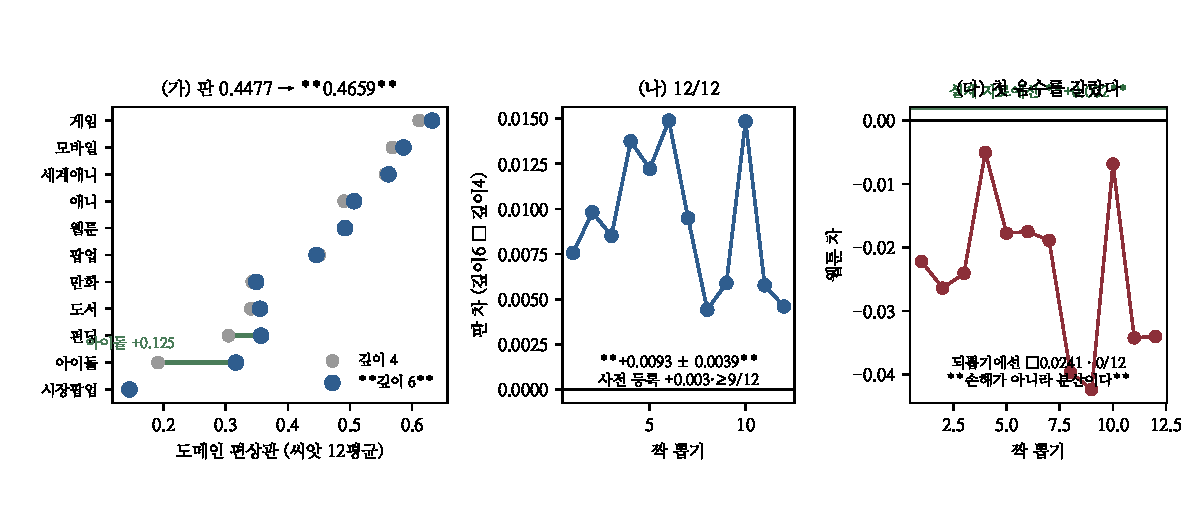
\includegraphics[width=\textwidth]{figs/fig406.pdf}
\caption{(가) 열한 도메인 전부. 아이돌이 $+0.125$ 로 제일 크게 오른다.
(나) 짝 12뽑기가 열둘 다 양수. (다) 웹툰 --- 되뽑기에선 $-0.0241 \cdot 0/12$
인데 실제 자료에선 $+0.002$ 다. 손해가 아니라 분산이다.}
\end{figure}

\end{document}
